\newpage
\section{Matrizen und lineare Abbildungen}
\subsection{Definition}
	Seien $V,W$ endlich dimensionale $K$-Vektorräume und $\mathcal{B}=\lrr{v_1,\dots,v_n}$ und\\
	$\varphi=\lrr{w_1,\dots,w_m}$ geordnete Basen von $V$ beziehungsweise $W$.\\
	Sei $\alpha: V\rightarrow W$ eine lineare Abbildung.\\
	Nach 4.10 ist $\alpha$ eindeutig bestimmt durch $\alpha\lrr{v_1},\dots,\alpha\lrr{v_n}$.\\
	Stelle $\alpha\lrr{v_1}$ bezüglich der BAsis $\varphi$ dar, $i=1,\dots,n$\\
	$\begin{array}{l}
		\alpha\lrr{v_1}=a_{11}w_1+\dots+a_{m1}w_m\\
		\vdots\\
		\alpha\lrr{v_n}=a_{1n}w_1+\dots+a_{mn}w_m
	\end{array}$\\
	Dann heißt die $m\times n$-Matrix \textbf{Darstellungsmatrix} von $\alpha$ bezüglich $\mathcal{B}$ und $\varphi$
	
	$A_{\alpha}^{\mathcal{B}, \varphi}:=\lrv{a_{11}&a_{12}&\dots&a_{1n}\\\vdots&\vdots&\dots&\vdots\\a_{m1}&a_{m2}&\dots&a_{mn}}$
	
	In den Spalten stehen die Koordinaten von $\alpha\lrr{v_i}$ bezüglich $\varphi, i=1,\dots,n$\\
	Beachte: Wenn $A_{\alpha}^{\mathcal{B}, \varphi}$ und $\mathcal{B},\varphi$ bekannt sind, dann ist $\alpha$ vollständig bestimmt.\\
	Abkürzende Schreibweise:\\
	$A_\alpha$ statt $A_{\alpha}^{\mathcal{B}, \varphi}$, wenn $\mathcal{B},\varphi$ aus Kontext ersichtlich sind.\\
	Falls $V=W$ und $\mathcal{B}=\varphi$: $A_{\alpha}^{\mathcal{B}}$ statt $A_{\alpha}^{\mathcal{B}, \mathcal{B}}$
	
\subsection{Beispiel}
	$V=W=\mr^2$, $\mathcal{B}$ ist kanonische Basis. $A_\alpha^{\mathcal{B}}=\lrv{1&2\\3&4}$\\
	Was ist $\alpha\lrr{\lrv{2\\3}}$?\\
	$\alpha\lrr{\lrv{1\\0}}=1\lrv{1\\0}+3\lrv{0\\1}=\lrv{1\\3}$\\
	$\alpha\lrr{\lrv{0\\1}}=\lrv{2\\4}$\\
	$\alpha\lrr{\lrv{2\\3}}=\alpha\lrr{2\cdot\lrv{1\\0}+3\cdot\lrv{0\\1}}=2\cdot\alpha\lrr{\lrv{1\\0}}+3\alpha\lrr{\lrv{0\\1}}=2\cdot\lrv{1\\3}+3\cdot\lrv{2\\4}=\lrv{8\\18}$
	
\subsection{Bemerkung}
	\subExBegin{a)}
		\item Nach 5.1 ist $\alpha$ durch $A_{\alpha}^{\mathcal{B}, \varphi}$ eindeutig bestimmt:\\
			$\mathcal{B},\varphi$ wie in 5.1, $\alpha:V\rightarrow W$.\\
			$v\in V, v=\limsum{i=1}{n}c_iv_i$, also ist\\
			$\alpha\lrr{v}=\limsum{i=1}{n}c_i\alpha\lrr{v_i}=\limsum{i=1}{n}c_i\lrr{\limsum{j=1}{m}a_{ji}w_j}=\limsum{j=1}{m}\underbrace{\lrr{\limsum{i=1}{n}a_{ji}c_i}}_{\mbox{\scriptsize Koord. }\scriptstyle \alpha(v)\mbox{\scriptsize \;bzgl. }\scriptstyle\varphi}w_j$
		\item Ist $A=\lrv{a_{11}&\dots&a_{1n}\\\vdots&&\vdots\\a_{m1}&\dots&a_{mn}}$ eine $m\times n$-Matrix über $K$.\\
			Dann existiert genau eine lineare Abbildung $\alpha:V\rightarrow W$ mit $A_{\alpha}^{\mathcal{B}, \varphi}=A$\\
			Das heißt jede $m\times n$-Matrix tritt als Darstellungsmatrix einer linearen Abbildung bezüglich vorgegebenen Basen $\mathcal{B}$ und $\varphi$ auf.
			
			Setze $w_i'=a_{1i}w_1+a_{2i}w_2+\dots+a_{mi}w{m}$, mit $i=1,\dots,n$, dann existiert nach 4.10 genau eine lineare Abbildung $\alpha:V\rightarrow W$ mit $\alpha\lrr{v_i}=w_i'$ für $i=1,\dots,n$\\
			Dann $A_{\alpha}^{\mathcal{B}, \varphi}=A$
		\item Dieselbe lineare Abbildung hat im Allgemeinen bezüglich anderer Wahl der Basen eine andere Darstellungsmatrix.
	\subExEnd
	
\subsection{Beispiele}
	\subExBegin{a)}
		\item $V=\mr^2=W, \mathcal{B}=\varphi$ kanonische Basis von $\mr^2$, $\alpha$ Drehung im Nullpunkt um den Winkel $\varphi$ gegen den Uhrzeigersinn.\\
			4.11:$\alpha\lrr{e_1}=\cos\lrr{\varphi}e_1+\sin\lrr{\varphi}e_2$\\
			$\alpha\lrr{e_2}=-\sin\lrr{\varphi}e_1+\cos\lrr{\varphi}e_2$
			
			$A_{\alpha}^{\mathcal{B}}=\underset{\mbox{\scriptsize Drehmatrix}}{\lrv{\cos\lrr{\varphi}&-\sin\lrr{\varphi}\\\sin\lrr{\varphi}&\cos\lrr{\varphi}}}$
		\item $\alpha:V\rightarrow W$ Nullabbildung hat bezüglich jeder Wahl von $\mathcal{B},\varphi$ die Nullmatrix als Darstellungsmatrix.
		\item $\mbox{id}_V:V\rightarrow V$, $\mathcal{B}$ Basis von $V$\\
			$A_{\mbox{id}_V}^{\mathcal{B}}=\lrv{1&0&\dots&0\\&&\\0&\dots&1}=E_n$ mit $\dim\lrr{V})n$
		\item zweidimensionales $V$ mit $\mathcal{v_1,v_2},\varphi=\lrv{v_2,v_1}$\\
			$A_{\mbox{id}_V}^{\mathcal{B},\varphi}=\lrv{0&1\\1&0}$
		\item $V=\mr^2,\mathcal{B}=\lrr{e_1,e_2}$ kanonische Basis, $\sigma$ Spiegelung an $\left\langle e_1\right\rangle$

      \begin{tikzpicture}[scale=1.5]
        \draw [-] (-2,0) -- (2,0);
        \draw [-] (0,-2) -- (0,2);
        \draw [thick,->] (0,0) -- (1,0) node [anchor=south west] {$e_1$};
        \draw [dotted] (1,-1) node [anchor=west] {$\sigma(v)$} -- (1,1) node [anchor=west] {$v$};
        \draw [thick,->] (0,0) -- (0,1) node [anchor=east] {$e_2$};
        \draw [thick,->] (0,0) -- (0,-1) node [anchor=east] {$-e_2$};
        \draw [->] (0,0) -- (1,1) node [anchor=south] {$\scriptstyle e_1+e_2$};
        \draw [->] (0,0) -- (1,-1) node [anchor=north] {$\scriptstyle e_1-e_2$};
      \end{tikzpicture}

			$A_{\sigma}^{\mathcal{B}}=\lrv{1&0\\0&-1}$\\
			$\sigma\lrr{\lrv{x_1\\x_2}}=\lrv{x_1\\-x_2}=\lrv{1&0\\0&-1}\lrv{x_1\\x_2}$\\
			$\mathcal{B}'=\lrr{e-1+e_2, e_1-e_2}=\lrr{\lrv{1\\1},\lrv{1\\-1}}$\\
			$A_\sigma^{\mathcal{B}'}=\lrv{0&1\\1&0}$\\
			$\sigma\lrr{e_1+e_2}=e_1-e_2=0\cdot\lrr{e_1+e_2}+1\cdot\lrr{e_1-e_2}$\\
			$\sigma\lrr{e_1-e_2}=e_1+e_2=1\cdot\lrr{e_1+e_2}+0\cdot\lrr{e_1-e_2}$

			$A_\sigma^{\mathcal{B},\mathcal{B}'}$\\
			$\sigma\lrr{e_1}=\underline{e_1}=a_{11}\lrr{e_1+e_2}+a_{21}\lrr{e_1-e_2}=\underline{\lrr{a_{11}+a_{21}}e_1+\lrr{a_{11}-a_{21}}e_2}$\\
			$\sigma\lrr{e_2}=\underline{-e_2}=a_{12}\lrr{e_1+e_2}+a_{22}\lrr{e_1-e_2}=\underline{\lrr{a_{12}+a_{22}}e_1+\lrr{a_{12}-a_{22}}e_2}$\\
			$a_{11}+a_{21}=1\quad a_{11}-a_{21}=0\Rightarrow a_{11}=a_{21}=\frac{1}{2}$\\
			$a_{12}+a_{22}=0\quad a_{12}-a_{22}=-1\Rightarrow a_{12}=-\frac{1}{2},a_{22}=\frac{1}{2}$\\
			$A_\sigma^{\mathcal{B},\mathcal{B}'}=\lrv{\frac{1}{2}&-\frac{1}{2}\\\frac{1}{2}&\frac{1}{2}}$
	\subExEnd

\subsection{Satz}
	$V,W$ sind endlich dimensionale $K$-Vektorräume, $\mathcal{B},\varphi$ geordnete Basen von $V$\\
	beziehungsweise $W$, $\alpha:V\rightarrow W$ eine lineare Abbildung.\\
	Sei $v\in V$, $k_{\mathcal{B}}\lrr{v}$ der Koordinatenvektro von $v$ bezüglich $\mathcal{B}$.\\
	Der Koordinatenvektor von $\alpha\lrr{v}$ bezüglich $\varphi$ lässt sich berechnen als\\
	$k_\varphi\lrr{\alpha\lrr{v}}=A_{\alpha}^{\mathcal{B},\varphi}\cdot k_\mathcal{B}\lrr{v}$

  \begin{tikzpicture}
    \draw [<-,thick] (0,0) node [anchor=north east] {$\scriptstyle K^n$} -- node [anchor=east] {$K_\mathcal{B}$} (0,2) node [anchor=south east] {$\scriptstyle\overset{\mathcal{B}}{V}$};
    \draw [->,thick] (0,2) -- node [anchor=south] {$\alpha$} (2,2) node [anchor=south west] {$\scriptstyle\overset{\varphi}{W}$};
    \draw [->,thick] (2,2) -- node [anchor=west] {$\scriptstyle K_l$} (2,0) node [anchor=north west] {$\scriptstyle K^m$};
    \draw [->,thick] (0,0) -- node [anchor=south] {$A_\alpha^{\mathcal{B},l}$} (2,0);
  \end{tikzpicture}

	\textbf{Beweis} - Folgt aus 5.3a)

\subsection{Beispiel}
	$V,W$ seien $\mr$-Vektorräume mit $\dim\lrr{V}=4, \dim\lrr{W}=3$ und $\mathcal{B}=\lrr{v_1,\dots,v_4},\varphi=\lrr{w_1,w_2,w_3}$, $\alpha:V\rightarrow W$ linear mit \\
	$A_\alpha^{\mathcal{B},\varphi}=\lrv{1&1&2&3\\2&0&-1&1\\3&2&0&2}$\\
	$v=5v-1-6v_2+7v_3-2v_4$, $\alpha\lrr{v}=?$\\
	5.5:$\lrv{1&1&2&3\\2&0&-1&1\\3&2&0&2}\lrv{5\\-6\\7\\-2}=\lrv{7\\1\\-1}$\\
	$\alpha\lrr{v}=7w_1+w_2-w_3$
	
\subsection{Korollar}
	Jede lineare Abbildung $K^n\rightarrow K^m$ ist von der Form $\alpha\lrr{x}=A\cdot x$ für eine $m\times n$-Matrix $A$ über $K$.
	
	%TODO - Yannick's part
